% Main Section: BAB II (unnumbered)

\section*{\centering BAB II \\ Gambaran Umum Instansi}

\addcontentsline{toc}{section}{BAB II Gambaran Umum Instansi}  % Manually add unnumbered section to ToC

% Set the section counter manually to "1" for subsections under BAB I
\setcounter{section}{2}
\setcounter{subsection}{0}  % Reset subsection
\setcounter{figure}{0}
\renewcommand{\thefigure}{\thesection.\arabic{figure}}

% Subsections under BAB II (numbered)
\subsection{Profil Organisasi}
Komisi Pemilihan Umum (KPU) Provinsi Lampung merupakan lembaga yang bertanggung jawab dalam menyelenggarakan pemilihan umum di tingkat provinsi. KPU Lampung menyelenggarakan pemilu untuk memilih anggota DPR, DPD, DPRD, Presiden dan Wakil Presiden, serta referendum \cite{KpuDefinition} .
\begin{figure}[h]
    \centering
    
\includegraphics[width=0.5\linewidth]{images/kpu_logo.png}
    \caption{Logo KPU Lampung}
    \label{fig:kpu_logo}
\end{figure}

\subsection{Visi dan Misi Organisasi}
Komisi Pemilihan Umum (KPU) Provinsi Lampung memiliki visi dan misi yang dijalankannya. Visi utamanya adalah “Menjadi Penyelenggara Pemilu Serentak yang Mandiri, Profesional dan Berintegritas”. Fokus utamanya adalah mendukung terciptanya organisasi Komisi Pemilihan Umum (KPU) Provinsi Lampung yang mampu melaksanakan tugas dan fungsinya dengan baik, disertai dengan kewibawaan dan kejujuran tanpa dipengaruhi oleh entitas lain dan memberikan layanan terbaik di bidang Pemilihan Umum dan Pemilihan \cite{VisiMisiKPU}. Selain itu Komisi Pemilihan Umum (KPU) Provinsi Lampung juga memiliki misi yang mencakup hal-hal berikut:
\begin{enumerate}
    \item Meningkatkan kompetensi penyelenggara Pemilu Serentak dengan berpedoman kepada perundang-undangan dan kode etik penyelenggara pemilu.
    \item Melaksanakan peraturan di bidang Pemilu Serentak yang memberikan kepastian hukum, progresif, dan partisipatif.
    \item Meningkatkan kualitas penyelenggaraan Pemilu Serentak yang efektif dan efisien, transparan, akuntabel, serta aksesibil.
    \item Mengoptimalkan pemanfaatan kemajuan teknologi informasi dalam menyelenggarakan Pemilu Serentak. 
    \item Meningkatkan partisipasi dan kualitas pemilih dalam Pemilu Serentak.
    \item Meningkatkan kualitas pelayanan Pemilu Serentak untuk seluruh pemangku kepentingan.
\end{enumerate}
 
\subsection{Struktur Organisasi}
\begin{figure}[h]
    \centering
    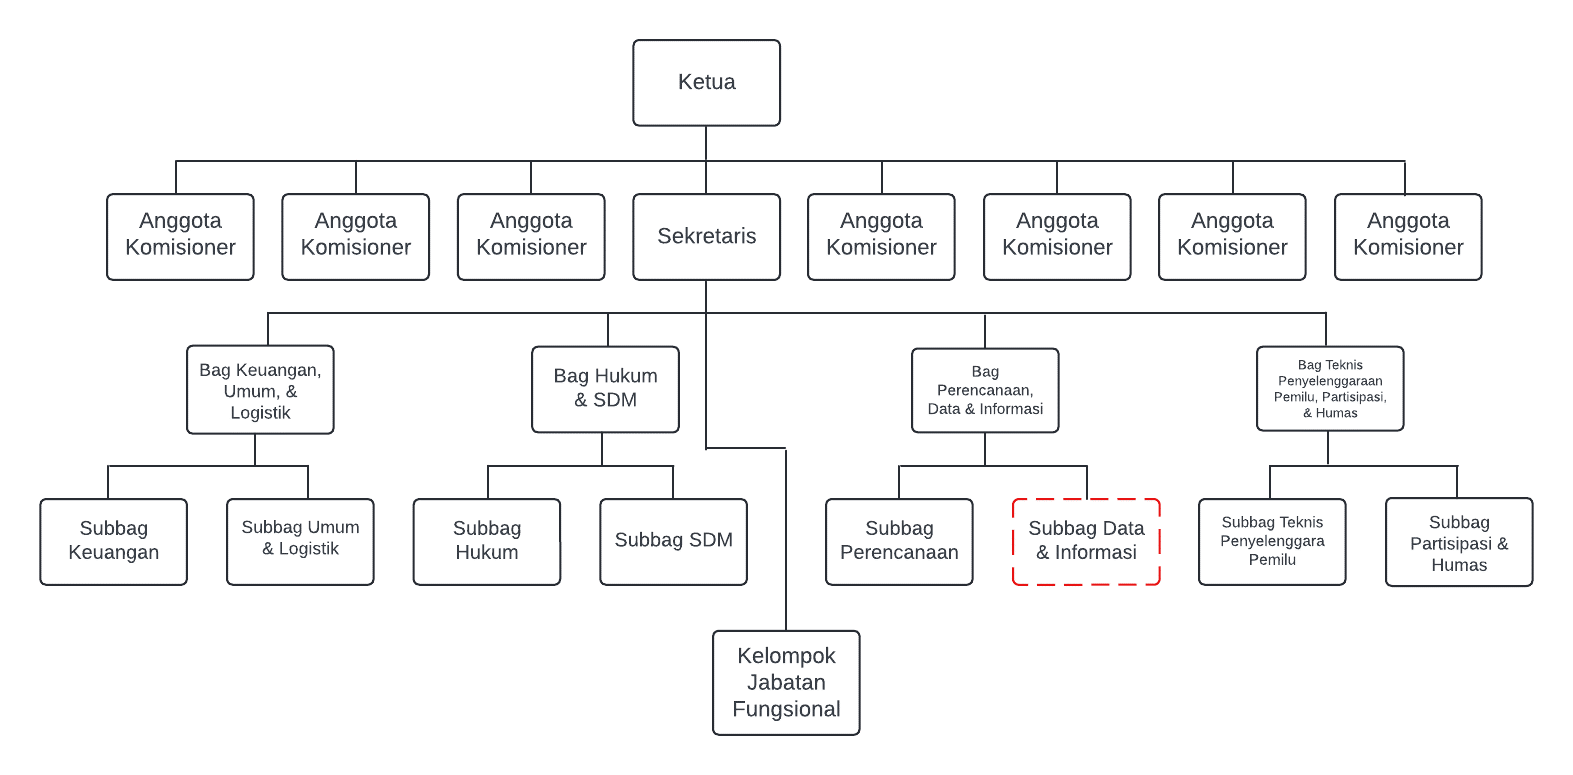
\includegraphics[width=1\linewidth]{images/kpu_struktur.png}
    \caption{Struktur KPU Provinsi Lampung}
    \label{fig:kpu_struktur}
\end{figure}

Struktur organisasi KPU Provinsi Lampung terdiri dari 7 tingkatan, yaitu Ketua KPU Provinsi Lampung, 7 Anggota Komisioner KPU Provinsi Lampung, Sekretaris KPU Provinsi Lampung, Kabag Keuangan, Umum, \& Logistik, Kabag Hukum \& SDM, Kabag Perencanaan, Data \& Informasi, dan Kabag Penyelenggaraan Pemilu, Partisipasi,\& Humas. Masing-masing tingkatan memiliki tugas dan fungsi yang berbeda-beda untuk memastikan penyelenggaraan pemilu yang transparan, akuntabel, dan berkualitas.

Ketua KPU Provinsi Lampung memimpin dan mengkoordinasikan pelaksanaan tugas dan fungsi KPU Provinsi Lampung. Anggota KPU Provinsi Lampung membantu Ketua KPU Provinsi Lampung dalam melaksanakan tugas dan fungsi KPU Provinsi Lampung. Sekretaris KPU Provinsi Lampung melaksanakan administrasi dan ketatausahaan KPU Provinsi Lampung. Kabag Keuangan, Umum, \& Logistik mengelola keuangan, umum, dan logistik KPU Provinsi Lampung. Kabag Hukum \& SDM mengelola hukum dan sumber daya manusia KPU Provinsi Lampung. Kabag Perencanaan, Data \& Informasi mengelola perencanaan, data, dan informasi KPU Provinsi Lampung. Kabag Penyelenggaraan Pemilu, Partisipasi, \& Humas menyelenggarakan pemilu, partisipasi masyarakat, dan hubungan masyarakat KPU Provinsi Lampung. Pada Praktek Kerja ini Saya ditempatkan di Divisi Data \& Informasi.

\subsection{Deskripsi Pekerjaan}
Dalam pelaksanaan kerja praktik di KPU Provinsi Lampung, penulis melakukan sebuah penelitian tentang klusterisasi pada data rekapitulasi data pemilih untuk Pilkada Provinsi Lampung 2024. Di sisi lain, penulis juga banyak membantu dan belajar mengenai administrasi di bagian Divisi Data dan Informasi KPU Provinsi Lampung.

Lingkup pekerjaan yang dilakukan oleh penulis adalah sebagai berikut:
\begin{enumerate}
    \item Melakukan kegiatan administrasi seperti membuat Surat Tugas, Surat Pertanggung Jawaban, dll dari kegiatan-kegiatan yang dilakukan oleh Divisi Data dan Informasi.
    \item Melakukan pengumpulan dan pengolahan data untuk klusterisasi data rekapitulasi daftar pemilih Pilkada 2024 Provinsi Lampung.
\end{enumerate}

\subsection{Jadwal Kerja}
Kegiatan kerja praktik dilakukan pada tanggal 19 Juni 2024 – 05 Agustus 2024 di KPU Provinsi Lampung. Pelaksanaan kerja praktik dilakukan selama Lima hari dalam satu minggu, yaitu pada hari Senin hingga hari Jumat. Untuk waktu pelaksanaan kerja praktik dimulai dari pukul 08.00 – 16.00 WIB. 

\newpage